\documentclass[tikz]{standalone}

\usepackage{tikz}
\usetikzlibrary{shapes.geometric, arrows}
\usetikzlibrary{positioning}
\usetikzlibrary{shapes.geometric,arrows,fit,matrix,shapes.multipart}
\usetikzlibrary{calc,shapes.arrows,decorations.pathreplacing,shadows}
\usetikzlibrary{arrows, arrows.meta, calc, positioning, quotes, shapes}
\usetikzlibrary{positioning, fit, arrows.meta, shapes}

\begin{document}


\begin{figure}[!htb]

\begin{flushleft}
Suppose we have a set of models $(\mathscr{M}_i)_{i=1}^k$, their parametrisations $(\theta_i)_{i=1}^k$, the assumed distributions of log returns for each model $(f_i)_{i=1}^k$, training data $(X_i)_{i=1}^m$ and validation data $(Y_j)_{j=1}^n$.
\end{flushleft}
\vspace{2mm}
\begin{flushleft}
    
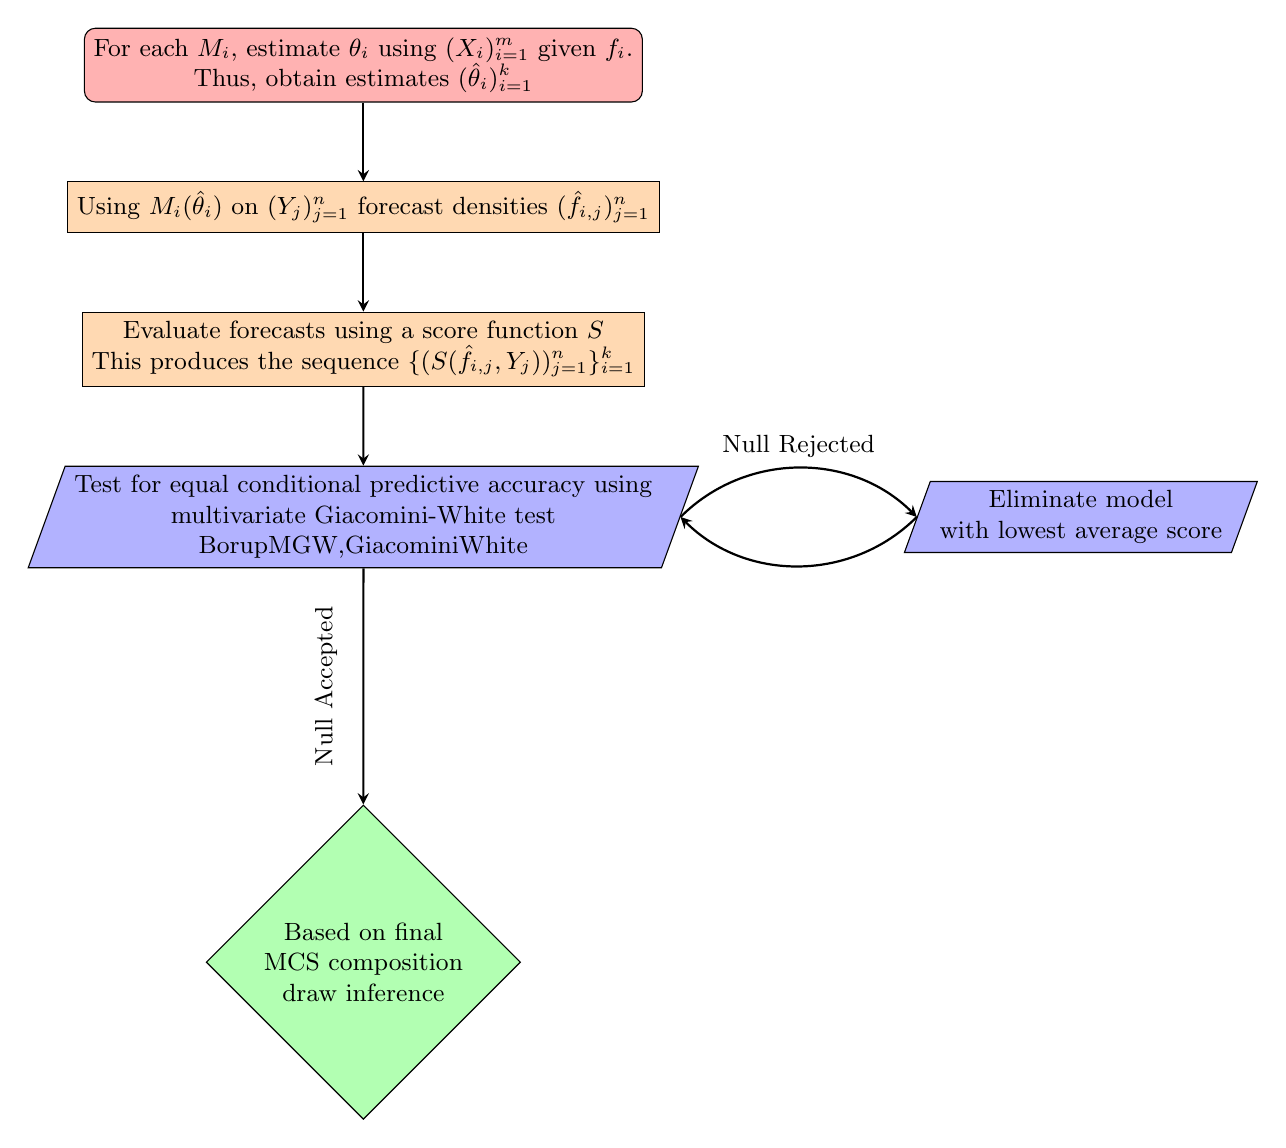
\begin{tikzpicture}[
    node distance = 1cm,
    arrow/.style={thick, ->, >=stealth},
      base/.style = {draw, minimum width=10mm, minimum height=5mm,
                     align=center},
 startstop/.style = {base, rounded corners, fill=red!30},
   process/.style = {base, fill=orange!30},
        io/.style = {base, trapezium, 
                     trapezium left angle=70, trapezium right angle=110,
                     fill=blue!30},
  decision/.style = {base, diamond, fill=green!30},
  every edge quotes/.style = {auto=right},
  font=\small]

\node (start) [startstop] {For each $\mathscr{M}_i$, estimate $\theta_i$ using $(X_i)_{i=1}^m$ given $f_i$. \\ Thus, obtain estimates $(\hat{\theta}_i)_{i=1}^k$};
\node (prediction) [process,below = of start] {Using $\mathscr{M}_i(\hat{\theta}_i)$ on $(Y_j)_{j=1}^n$ forecast densities $(\hat{f}_{i,j})_{j=1}^n$};
\node (evaluation) [process,below = of prediction] {Evaluate forecasts using a score function $S$ \\ This produces the sequence $\{(S(\hat{f}_{i,j},Y_j))_{j=1}^n\}_{i=1}^k$};
\node (MCS1) [io, below= of evaluation] {Test for equal conditional predictive accuracy using \\ multivariate Giacomini-White test \\ \citep{BorupMGW,GiacominiWhite} };
\node (MCS2) [io,right = 3cm of MCS1] {Eliminate model \\ with lowest average score};
\node (Inference) [align=center,decision, below= 30mm of MCS1] {Based on final \\ MCS composition \\ draw inference};

\draw [arrow] (start) -- node[anchor=north] {} (prediction);
\draw [arrow] (prediction) -- node[anchor=north] {} (evaluation);
\draw [arrow] (evaluation) -- node[anchor=north] {} (MCS1);
\draw [arrow] (MCS1.east) to [anchor=east,bend left=45]  node [anchor=east,above, sloped]  (TextNode2) {Null Rejected} (MCS2.west);
\draw [arrow] (MCS2.west) to [anchor=east,bend left=45]  node [anchor=east,above, sloped]  (TextNode2) {} (MCS1.east);
\draw [arrow] (MCS1) -- node[anchor=north, above=2mm, sloped] {Null Accepted} (Inference);



\end{tikzpicture}
\end{flushleft}
\caption{Organisation of Methodology}\label{Methodology Diagram}
\end{figure}

\end{document}{
